\documentclass[11pt]{report} % use larger type; default would be 10pt

\usepackage[utf8]{inputenc} % set input encoding (not needed with XeLaTeX)


%%% PAGE DIMENSIONS
\usepackage{geometry} % to change the page dimensions
\geometry{letterpaper} % or letterpaper (US) or a5paper or....
\geometry{margin=0.75in} % for example, change the margins to 2 inches all round
% \geometry{landscape} % set up the page for landscape
%   read geometry.pdf for detailed page layout information

%%% PACKAGES
\usepackage{datetime} % for date without day
\usepackage{graphicx} % support the \includegraphics command and options
\usepackage{epstopdf}
\usepackage{amsmath,amssymb,amsthm}
\usepackage{mathrsfs}                      % Gives us \mathscr for \setset
\usepackage{wrapfig}
\usepackage{array}
\usepackage[table]{xcolor}
\usepackage{booktabs}
\usepackage{titlesec}
\usepackage[normalem]{ulem}
\newcommand{\subfigureautorefname}{\figureautorefname}
\usepackage{chemarr}
\usepackage{listings}
\definecolor{Gray}{gray}{0.85}
\newdateformat{monthyeardate}{\monthname[\THEMONTH], \THEYEAR} % new date format
\newcommand{\ra}[1]{\renewcommand{\arraystretch}{#1}}
\newcolumntype{L}[1]{>{\raggedright\let\newline\\\arraybackslash\hspace{0pt}}m{#1}}
\newcolumntype{C}[1]{>{\centering\let\newline\\\arraybackslash\hspace{0pt}}m{#1}}
\newcolumntype{R}[1]{>{\raggedleft\let\newline\\\arraybackslash\hspace{0pt}}m{#1}}
\usepackage{indentfirst}
\usepackage[hidelinks]{hyperref}
\hypersetup{
	colorlinks,
	linkcolor={blue!50!black},
	citecolor={blue!50!black},
	urlcolor={blue!80!black}
}
% for writing algorithms
\usepackage{algpseudocode}
\usepackage{algorithm}

\makeatletter
\newcommand{\removelatexerror}{\let\@latex@error\@gobble}
\makeatother

\usepackage{booktabs} % for much better looking tables
\usepackage{array} % for better arrays (eg matrices) in maths
\usepackage{paralist} % very flexible & customisable lists (eg. enumerate/itemize, etc.)
\usepackage{verbatim} % adds environment for commenting out blocks of text & for better verbatim
\usepackage{subfig} % make it possible to include more than one captioned figure/table in a single float
% These packages are all incorporated in the memoir class to one degree or another...

%%% HEADERS & FOOTERS
\usepackage{fancyhdr} % This should be set AFTER setting up the page geometry
\pagestyle{fancy} % options: empty , plain , fancy
\renewcommand{\headrulewidth}{0pt} % customise the layout...
\lhead{}\chead{}\rhead{}
\lfoot{}\cfoot{\thepage}\rfoot{}

%%% SECTION TITLE APPEARANCE
\usepackage{sectsty}
%\allsectionsfont{\sffamily\mdseries\upshape} % (See the fntguide.pdf for font help)
% (This matches ConTeXt defaults)


%%% ToC (table of contents) APPEARANCE
\usepackage[nottoc,notlof,notlot]{tocbibind} % Put the bibliography in the ToC
\usepackage[titles,subfigure]{tocloft} % Alter the style of the Table of Contents
\renewcommand{\cftsecfont}{\rmfamily\mdseries\upshape}
\renewcommand{\cftsecpagefont}{\rmfamily\mdseries\upshape} % No bold!

%%% New commands%%%%%
\setcounter{secnumdepth}{4}
\titleformat{\paragraph}
{\normalfont\normalsize\bfseries}{\theparagraph}{1em}{}
\titlespacing*{\paragraph}
{0pt}{3.25ex plus 1ex minus .2ex}{1.5ex plus .2ex}

\addtocontents{loa}{\def\string\figurename{Algorithm}} % list of algorithms

%%%%%%%%% Javascript for listing %%%%%%%%%%%%%%%%%%%
\lstdefinelanguage{JavaScript}{
	keywords={typeof, new, true, false, catch, function, return, null, catch, switch, var, if, in, while, do, else, case, break},
	keywordstyle=\color{blue}\bfseries,
	ndkeywords={class, export, boolean, throw, implements, import, this},
	ndkeywordstyle=\color{darkgray}\bfseries,
	identifierstyle=\color{black},
	sensitive=false,
	comment=[l]{//},
	morecomment=[s]{/*}{*/},
	commentstyle=\color{purple}\ttfamily,
	stringstyle=\color{red}\ttfamily,
	morestring=[b]',
	morestring=[b]"
}

\lstset{
	language=JavaScript,
	backgroundcolor=\color{white},
	extendedchars=true,
	basicstyle=\footnotesize\ttfamily,
	showstringspaces=false,
	showspaces=false,
	numbers=left,
	numberstyle=\footnotesize,
	numbersep=9pt,
	tabsize=2,
	breaklines=true,
	showtabs=false,
	captionpos=b
}
%%%%%%%%%%%%%%%%%%%%%%%%%%%%%%%%%%%%%%%%%%%%%%%%%%%%%%%%%%%%%%%%%%%%%%%%%%%%%%%%%%%%%%


%%%%%%%%% Jason for listing %%%%%%%%%%%%%%%%%%%
\lstdefinelanguage{json}{
	basicstyle=\normalfont\ttfamily,
	numbers=left,
	numberstyle=\scriptsize,
	stepnumber=1,
	numbersep=8pt,
	showstringspaces=false,
	breaklines=true,
%	frame=lines,
	backgroundcolor=\color{white},
}

%%%%%%%%%%%%%%%%%%%%%%%%%%%%%%%%%%%%%%%%%%%%%%%%%%%%%%%%%%%%%%%%%%%%%%%%%%%%%%%%%%%%%%

%%% GRAPHICS PATH
%\graphicspath{{E:/DissertationProspectus/figures/}}

%%% END Article customizations

%%% The "real" document content comes below...

\begin{document}
	
	%Title Page
	\thispagestyle{empty}
	\begin{center}
		\begin{minipage}{\linewidth}
			\centering
			%Thesis Title
			\vspace{2cm}
			{\Huge \bf{Voice Command Browsing (Extension for Google Chrome  Browser)}\par}
			\vspace{1cm}
			%Report type		
			{\Large \bfseries{MINI PROJECT REPORT}\par}
			\vspace{0.5cm}
			{\Large \emph{Submitted in partial fulfillment of the requirements for the award of degree}\par}
			\vspace{0.5cm}
			{\Large \bf{BACHELOR OF TECHNOLOGY} \par}
			\vspace{0.5cm}
			{\Large \bf{BY} \par}
			\vspace{1cm}
			%Author's name
			{\Large \bf{RAJESH R NAIR}\hspace{3cm}     Reg.no:14015695 \par}
			{\Large \bf{UNNIKRISHNAN}\hspace{3cm}      Reg.no:14015716 \par}
			\vspace{1cm}
			% logo							
			
\includegraphics[width=0.5\linewidth]{figures/logo.png}
			
			%School
			{\Large \bfseries{SCMS SCHOOL OF ENGINEERING AND TECHNOLOGY}\par}
			{\Large \emph{(Affiliated to M.G. University)}\par}
			{\Large VIDYA NAGAR, PALISSERY, KARUKUTTY\par}
			{\Large ERNAKULAM – 683 582\par}
			\vspace{1cm}
			
			%\vspace{2cm}
			
			%Date
			{\Large \monthyeardate \today}
		\end{minipage}
	\end{center}
	\clearpage
	
	
	% Certificate page
	\thispagestyle{empty}
	\begin{center}
		\begin{minipage}{\linewidth}
			\centering
			%\vspace{1cm}			
			% logo					
			
\includegraphics[width=0.5\linewidth]{figures/logo.png}
			\vspace{1cm}
			%School
			\\
			
			{\Large \bf{SCMS SCHOOL OF ENGINEERING AND TECHNOLOGY}\par}
			{\Large \emph{(Affiliated to M.G. University)}\par}
			{\Large VIDYA NAGAR, PALISSERY, KARUKUTTY\par}
			{\Large ERNAKULAM – 683 582\par}
			\vspace{1cm}
			{\Large \bf{\underline{BONAFIDE CERTIFICATE}}\par}
			\vspace{0.5cm}
			\begin{flushleft}
				This is to certify that the mini project, titled ''Voice Command Browsing (Extension for Google Chrome  Browser)'' by
			\end{flushleft} 
			%\vspace{0.5cm}
			%Author's name
			{ \bf{RAJESH R NAIR}\hspace{3cm}     Reg.no:14015695 \par}
			{ \bf{UNNIKRISHNAN}\hspace{3cm}      Reg.no:14015716 \par}
			\begin{flushleft}
				submitted in partial fulfilment of the requirement for the award of the degree of Bachelor of Technology, is a bonafide work carried under supervision, during the academic year 2015-2016.
			\end{flushleft}
		    \vspace{2cm}
			{ \bf{Ms. DEEPA SREE VARMA}\hspace{3.5cm}     Prof. VINOD P \par}
			{ \bf{PROJECT GUIDE}\hspace{3cm}      HEAD OF DEPARTMENT\par}
			
			\vspace{3cm}
			
			{ \bf{INTERNAL EXAMINER}\hspace{3cm}     EXTERNAL EXAMINER \par}
			
			
		\end{minipage}
	\end{center}
	\clearpage
	
	
	
	
	%Abstract Page
	\thispagestyle{empty}
	\begin{center}
		\begin{minipage}{\linewidth}
			\vspace{3cm}
			{\centering \bf{Abstract}\par}
			\vspace{0.5cm}
			Surfing the internet has reached the top in the list of things done for entertainment in the world on a daily basis. As such browsers used for this purpose have unintentionally become the most used applications on a desktop or laptop. 
			Browsing trends have evolved over the years, from the default used text searches to speech recognition based search and even image based search across the web. 
			The goal of this project is to create a vocal command based extension which can be used to perform the basic and a few intermediate functions that are otherwise done in the browser using the keyboard or mouse. 
			For instance, voice commands can be given to open a new tab rather than doing so using a mouse. A variety of such simple commands can be implemented to improve the functionalities of the extension.
			The goal of this project is to design and implement a extension or an add-on which performs functions based on simple voice commands. The extension will be set to work on any Google Chrome browser. The extension will be made available in the Google Chrome support page (which has all extensions and extensions). 
			The users can install it and make it available on their Google Chrome browser.  
			The project aims to improve the ease of accessibility of Google Chrome browser users using voice commands rather than the usual type-and-click method. 
			Users will be free to leave their keyboards and mouse and can depend on just their own voices to perform most browser related operations such as opening a new tab, closing tabs, searching the web etc. Though no functions in websites itself can be performed, the browser related operations will be easily done using this extension. 
		\end{minipage}
	\end{center}
	\clearpage
	
	
	%ACKOWLEDGEMENT Page
	\thispagestyle{empty}
	\begin{center}
		\begin{minipage}{\linewidth}
			\vspace{3cm}
			{\centering \bf{ACKOWLEDGEMENT}\par}
			\vspace{0.5cm}
			We are greatly indebted to Prof.M.Madhavan, Principal, SSET, Ernakulam and Prof.Vinod, Head of department, Department of Computer Science and Engineering, SSET, who whole heartedly granted us the permission to carry out the mini project.
			We would like to thank our guide, Ms.Deepa Sree Varma, Assistant Professor, Department of  Computer Science and Engineering, SSET who has given us valuable guidance and support throughout the project. Also, we would like to thank our project coordinators, Ms.Shilpa  P C and Ms.Gayathri  Assistant Professors, Department of Computer Science and Engineering, SSET, who supported and instructed us all the way.
			We would like to express our sincere gratitude to all the teachers of Computer Science Department who gave us moral and technical support through the course of our mini project. We would like to thank the supporting staff in the Computer lab whose dedicated work kept the lab working smoothly, thus ensuring our time at the lab went hassle free.
			
		\end{minipage}
	\end{center}
	\clearpage
	
	\tableofcontents
	\listoffigures
	\listoftables
	\newpage

\chapter{Introduction}
\label{chap:Intro}



\section{OVERVIEW}
\label{sec:OVERVIEW}
The 'Voice Enabled browser' consists of three main parts: Speech Engine , the Java application and the Interface. The relationships between the modules can be seen in the following simplified class diagram. The GUI is the part of Interface module of the project.  The speech recognizer will listen to what you say and convert your words to a string. A voice browsing extension is a software application that presents an interactive voice user interface to the user in a manner analogous to the functioning of a web browser interpreting Hypertext Markup Language (HTML). Dialog documents interpreted by browser are often encoded in standards-based markup languages, such as Voice Dialog Extensible Markup Language (VoiceXML), a standard by the World Wide Web Consortium. A voice browser presents information aurally, using pre-recorded audio file playback or text-to-speech synthesis software. A voice browser obtains information using speech recognition \cite{Ornbospeech,Walshspeech,speechStackoverflow} and keypad entry, such as DTMF detection. As speech recognition and web technologies have matured, voice applications are deployed commercially in many industries and voice browsers are supplanting traditional proprietary interactive voice response (IVR) systems. Voice browser software is delivered in a variety of implementations models.


\section{PROBLEM ANALYSIS}
\label{sec:PROBLEM ANALYSIS}

Problem analysis is the process of understanding the actual problems, user needs and proposing solutions to meet those needs. The goal of problem analysis is to gain a better understanding of the problem being solved before development begins. It is the process of gathering and interpreting facts, diagnosing problems and using the information to recommend improvements on the system. Problem analysis is problem solving activities that require intensive communication between users and the system developers. A problem can be defined as the difference between things as perceived and things as desired. The system is studied and analyzed. The system is viewed as a whole and the input to the system are identified. The output from the system is given to various processes.


\section{EXISTING SYSTEM}
\label{sec:EXISTING SYSTEM}

\subsection{KEYBOARD}
\label{subsec:KEYBOARD} 
In normal usage, the keyboard is used as a text entry interface to type text and numbers into a word processor, text editor or other programs. In a modern computer, the interpretation of key presses is generally left to the software. A computer keyboard distinguishes each physical key from every other and reports all key presses to the controlling software. Keyboards are also used for computer gaming, either with regular keyboards or by using keyboards with special gaming features, which can expedite frequently used keystroke combinations.

\subsection{MOUSE}
\label{subsec:MOUSE}
A computer mouse is a pointing device (hand control) that detects two-dimensional motion relative to a surface. This motion is typically translated into the motion of a pointer on a display, which allows a smooth control of the graphical user interface.
Physically, a mouse consists of an object held in one's hand, with one or more buttons. Mice often also feature other elements, such as touch surfaces and "wheels", which enable additional control and dimensional input.

\section{PROPOSED SYSTEM}
\label{sec:PROPOSED SYSTEM}
Aims to improve the ease of accessibility of chrome browser users using voice commands rather than the usual type-and-click method.
A vocal command based extension which can be used to perform the basic and a few intermediate functions that are otherwise done in the browser using the keyboard or mouse.
Users will be free to leave their keyboards and mouses and can depend on just their own voices to perform most browser related operations such as opening a new tab, closing tabs, searching the web etc. 

\section{FEASIBILITY STUDY}
\label{sec:FEASIBILITY STUDY}

Feasibility study is a procedure that identifies, describes and evaluates candidate systems and selects the best system for the job. An estimate is made whether the identified users need may be satisfied using the current software and hardware technologies. The study will decide whether the proposed system will be cost effective from a business point of view and if it can be developed using the given existing budgetary constraints. 
The key considerations involved in the feasibility analysis are the following:


\begin{enumerate}
	\item Economic feasibility
	\item Technical feasibility
	\item Operational feasibility
\end{enumerate}


\subsection{ECONOMIC FEASIBILITY}
\label{subsec:ECONOMIC FEASIBILITY}

Economic study is the most frequently used method for evaluating the effectiveness of candidate system. More commonly known as cost/benefit analysis, the procedure is to determine the benefits and savings that are accepted from a candidate system and compares with costs. If benefit outweighs cost, then decisions are made to design and implement the system. Otherwise further alterations will have to be made if to have a chance of being approved.
Less hardware is required and can also be mounted on the existing wheelchair with reduced complexity.Hence this project is economically feasible and is cost effective because of its compatibility and effort saving nature.


\subsection{TECHNICAL FEASIBILITY}
\label{subsec:TECHNICAL FEASIBILITY}

Technical feasibility is a measure of how feasible the project is technically. The effort and technology included in the conventional system is not needed as the whole process is automated.
The hierarchy of the new system is very easier than the existing system. The new system is very much easier and user friendly. Operational cost is very easy. The maintenance and modification of the new system needs very less human effort. 


\subsection{OPERATIONAL FEASIBILITY}
\label{subsec:OPERATIONAL FEASIBILITY}
Its is very reliable since a microphone is supported by all existing systems and the voice recognition system enables the user to save time by using simple commands instead of typing externally .this facility doesnot  require  any preexperience since all included invoking commands are simple names which is common to all.


\chapter{DESIGN}
\label{cha:DESIGN}


\section{BLOCK DIAGRAM}
\label{sec:DATA FLOW DIAGRAMS}

\subsection{CONTEXT LEVEL DFD}
\label{subsec:CONTEXT LEVEL DFD}

\begin{figure}[h]
	\centering
	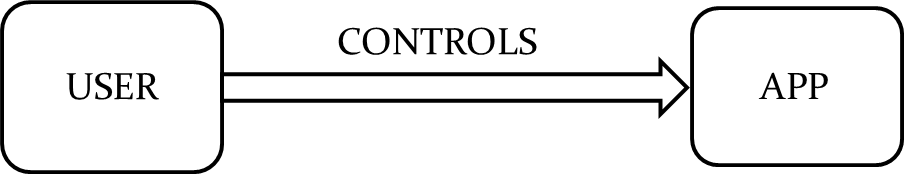
\includegraphics[width=0.5\linewidth]{figures/context_level_DFD.png}
	\caption{Context level DFD}
	\label{fig:Context level DFD}
\end{figure}


\begin{enumerate}
	\item Context level DFD shown in \autoref{fig:Context level DFD} is the most basic representation of the system.
	\item This indicates the basic working of the system.
	\item The user controls the application.
\end{enumerate}


\subsection{LEVEL 0 DFD}
\label{subsec:LEVEL 0 DFD}
\begin{figure}[h]
	\centering
	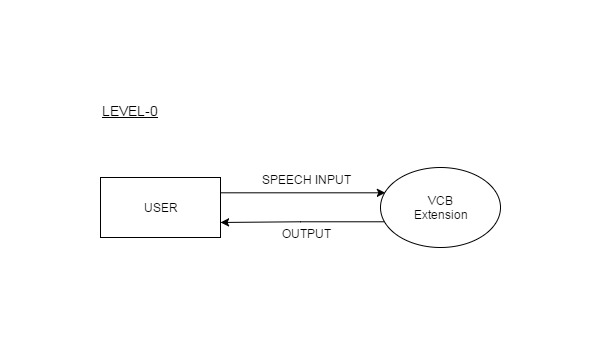
\includegraphics[width=0.5\linewidth]{figures/DFD0.jpg}
	\caption{Level 0 DFD}
	\label{fig:Level 0 DFD}
\end{figure}

\begin{enumerate}
	\item Level 0 DFD shown in \autoref{fig:Level 0 DFD} indicates the basic processes involved in the system.
	\item This level indicates all the processes of our system.
\end{enumerate}

\subsection{LEVEL 1 DFD}
\label{subsec:LEVEL 1 DFD}
\begin{figure}[h]
	\centering
	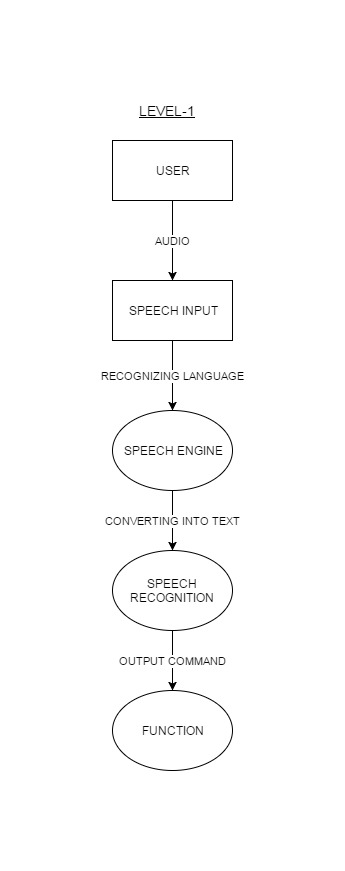
\includegraphics[width=0.5\linewidth, height=.8\linewidth]{figures/DFD1.jpg}
	\caption{Level 1 DFD}
	\label{fig:DFD1}
\end{figure}

\begin{enumerate}
	\item Level 1 DFD shown in \autoref{fig:DFD1} represents working of the extension
\end{enumerate}

\subsection{LEVEL 2 DFD}
\label{subsec:LEVEL 2 DFD}
\begin{figure}[h]
	\centering
	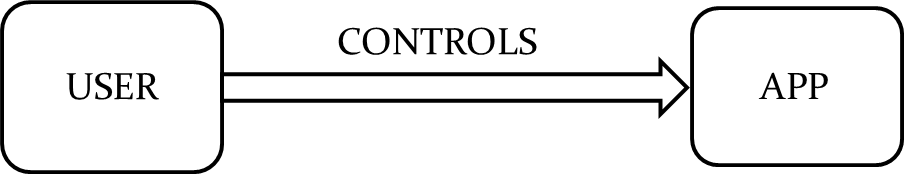
\includegraphics[width=0.5\linewidth]{figures/DFD2.png}
	\caption{Level 2 DFD}
	\label{fig:DFD2}
\end{figure}

\begin{enumerate}
	\item Level 2 shown in \autoref{fig:DFD2} includes the processing in speech api which fetch data from the server.
\end{enumerate}

%\section{TABLE}
%\label{sec:TABLE}
%
%\subsection{ITEMS}
%\label{subsec:ITEMS}


\chapter{IMPLEMENTATION}

\section{SYSTEM REQUIREMENTS}
\label{sec:SYSTEM REQUIREMENTS}


\subsection{HARDWARE REQUIREMENTS}
\label{subsec:HARDWARE REQUIREMENTS}
Requirements that helps in communication between the Android app and the hardware
\begin{itemize}
	\item Laptop i5-6200 1tb HDD and 8gb RAM
	\item Laptop i5-6200 1tb HDD and 4gb RAM
	\item Microphone
\end{itemize}

\subsection{SOFTWARE REQUIREMENTS}
\label{subsec:SOFTWARE REQUIREMENTS}
Requirements that helps in developing the software
\begin{itemize}
	\item Online Database Storage
	\item Windows 7/8/10
	\item Wifi Connectivity
	\item Java script
	\item Chrome Browser
\end{itemize}
\section{PLATFORM AND IDE}
\label{sec:PLATFORM AND IDE}


\subsection{ONLINE DATABASE STORAGE}
\label{subsec:ONLINE DATABASE STORAGE}
Online data storage refers to the practice of storing electronic data with a third party service accessed via the Internet. It is an alternative to traditional local storage (such as disk or tape drives) and portable storage (such as optical media or flash drives). It can also be called "hosted storage,""Internet storage" or "cloud storage."
In recent years, the number of vendors offering online data storage for both consumers and businesses has increased dramatically. Some services store only a particular kind of data, such as photos, music or backup data, while others will allow users to store any type of file. Most of these vendors offer a small amount of storage for free with additional storage capacity available for a fee, usually paid on a monthly or annual basis.

\subsection{WINDOWS}
\label{subsec:WINDOWS}
Microsoft Windows (or simply Windows) \cite{Maluth:2012:MWG:2464833} is a metafamily of graphical operating systems developed, marketed, and sold by Microsoft. It consists of several families of operating systems, each of which cater to a certain sector of the computing industry with the OS typically associated with IBM PC compatible architecture. Active Windows families include Windows NT and Windows Embedded; these may encompass subfamilies, e.g. Windows Embedded Compact (Windows CE) or Windows Server. Defunct Windows families include Windows 9x, Windows Mobile and Windows Phone.
Microsoft introduced an operating environment named Windows on November 20, 1985, as a graphical operating system shell for MS-DOS in response to the growing interest in graphical user interfaces (GUIs). Microsoft Windows came to dominate the world's personal computer (PC) market with over 90\% market share, overtaking Mac OS, which had been introduced in 1984. Apple came to see Windows as an unfair encroachment on their innovation in GUI development as implemented on products such as the Lisa and Macintosh (eventually settled in court in Microsoft's favor in 1993). On PCs, 
Windows is still the most popular operating system. However, in 2014, Microsoft admitted losing the majority of the overall operating system market to Android, because of the massive growth in sales of Android smartphones. In 2014, the number of Windows devices sold was less than 25\% that of Android devices sold. This comparison however may not be fully relevant, as the two operating systems traditionally target different platforms.
As of September 2016, the most recent version of Windows for PCs, tablets, smartphones and embedded devices is Windows 10. The most recent versions for server computers is Windows Server 2016. A specialized version of Windows runs on the Xbox One game console.

\subsection{WIFI CONNECTIVITY}
\label{subsec:WIFI CONNECTIVITY}
Wi-Fi or WiFi is a technology for wireless local area networking with devices based on the IEEE 802.11 standards. Wi-Fi is a trademark of the Wi-Fi Alliance, which restricts the use of the term Wi-Fi Certified to products that successfully complete interoperability certification testing.
Devices that can use Wi-Fi technology include personal computers, video-game consoles, smartphones, digital cameras, tablet computers, digital audio players and modern printers. Wi-Fi compatible devices can connect to the Internet via a WLAN network and a wireless access point. Such an access point (or hotspot) has a range of about 20 meters (66 feet) indoors and a greater range outdoors. Hotspot coverage can be as small as a single room with walls that block radio waves, or as large as many square kilometers achieved by using multiple overlapping access points.
Depiction of a device sending information wirelessly to another device, both connected to the local network, in order to print a document
Wi-Fi most commonly uses the 2.4 gigahertz (12 cm) UHF and 5 gigahertz (6 cm) SHF ISM radio bands. Having no physical connections,it is more vulnerable to attack than wired connections, such as Ethernet.

\subsection{JAVASCRIPT}
\label{subsec:JAVASCRIPT}
JavaScript \cite{JavascriptTutorialspoint,powell2004javascript}  often abbreviated as "JS", is a high-level, dynamic, untyped, interpreted run-time language. It has been standardized in the ECMAScript language specification. Alongside HTML\cite{htmlW3schools} and CSS\cite{cssW3schools}, JavaScript is one of the three core technologies of World Wide Web content production; the majority of websites employ it, and all modern Web browsers support it without the need for plug-ins\cite{Ahmed:2014:WDP:2675602}. JavaScript is prototype-based with first-class functions, making it a multi-paradigm language, supporting object-based, imperative, and functional programming styles.It has an API for working with text, arrays, dates and regular expressions, but does not include network, storage, or graphics APIs, relying instead upon APIs made available by its host environment\cite{js_validation_apiW3schools} .
Although there are strong outward similarities between JavaScript and Java, including language name, syntax, and respective standard libraries, the two languages are distinct and differ greatly in design; JavaScript was influenced by programming languages such as Self and Scheme.
JavaScript is also used in environments that are not Web-based, such as PDF documents, site-specific browsers, and desktop widgets. Newer and faster JavaScript virtual machines (VMs) and platforms built upon them have also increased the popularity of JavaScript for server-side Web applications. On the client side, developers have traditionally implemented JavaScript as an interpreted language, but more recent browsers perform just-in-time compilation. Programmers also use JavaScript in video-game development and in desktop and mobile applications.

\subsection{GOOGLE CHROME BROWSER}
\label{subsec:GOOGLE CHROME BROWSER}
Google Chrome is a freeware web browser developed by Google, It was first released in 2008, for Microsoft Windows, and was later ported to Linux\cite{Siever:2005:LN:1212560} , macOS, iOS and Android. Google Chrome is also the main component of Chrome OS, where it serves as a platform for running web apps \cite{chromeExtension}.
Google releases the majority of Chrome's source code as the Chromium open-source project.A notable component that is not open-source is the built-in Adobe Flash Player (that Chrome has disabled by default since September 2016). Chrome used the WebKit layout engine until version 27. As of version 28, all Chrome ports except the iOS port use Blink, a fork of the WebKit engine.
As of February 2017, StatCounter estimates that Google Chrome has a 62\% worldwide usage share of web browsers as a desktop browser. It also has 52\% market share across all platforms combined,because it is also the most popular browser for smartphones. Its success has led to Google expanding the "Chrome" brand name on various other products such as Chromecast, Chromebook, Chromebit, Chromebox and Chromebase.


\section{DETAILS OF IMPLEMENTATION}
\label{sec:DETAILS OF IMPLEMENTATION}

The main objective of our project is to design a wheelchair that will be controlled wirelessly and will be very easy to operate it with no physical efforts.Implementation is the stage of the project when the theoretical design is turned out into a working system. Thus it can be considered to be the most critical stage in achieving a successful new system and in giving the user, confidence that the new system will work and be effective.
The implementation stage involves careful planning, investigation of the existing system and it's constraints on implementation, designing of methods to achieve changeover and evaluation of changeover methods.

\subsection{SOURCE CODE}
\label{subsec:SOURCE CODE}
\subsubsection{Javascript code}
\label{subsubsec:Javascript code}
\lstinputlisting{code/tab.js}
\subsubsection{Json code}
\label{subsubsec:Json code}
\lstinputlisting[language=json]{code/manifest.json}
\subsubsection{HTML code}
\label{subsubsec:HTML code}
\lstinputlisting[language=HTML]{code/jj.html}


\chapter{TESTING}
\label{cha:TESTING}

Testing is the most important activity in the development phase. Testing is the process of    finding   errors or bugs in the system. Testing ensuresthe satisfaction of the users. In other words it isprocess by which one detects the defects in the system. Software testing methods are  traditionally divided into black box testing and white box testing. These two approaches are used to describe the point of view that a test engineer takes when designing test cases.

\section{TEST PLANS}
\label{sec:TEST PLANS}

The implementation of a computer-based system requires that test data can be prepared and that the system and its elements be tested in a planned, structured manner. The computer program component is a major subsystem of the computer-based information system, and particular attention should be given to the testing of these system elements as it is developed.
Testing is a process of executing a program with the interest of finding an error. A good test is one that has a high probability of finding the yet undiscovered errors. The primary objective for the test case design is to drive a set of tests that has the highest likelihood for systematically uncovering different classes of errors in the software. A series of testing are performed for this project before the system is ready for acceptance.  Some of the testing strategies applied for the system are listed here.

Testing Strategies: 
\begin{enumerate}
	\item Black Box Testing
	\item White Box Testing
\end{enumerate}

\subsection{Black Box Testing}
\label{subsec:Black Box Testing}

Black Box testing also called functional testing, focuses on the functional requirements of the software. Knowing the specified function that a product designed to perform the test can be conducted to ensure that each function is fully operational. Black Box tests are carried out to test that input to function is properly accepted and output is correctly produced. It finds the errors in the following categories:

\begin{enumerate}
	\item Interface errors.
	\item Performance in data structures or external database access.
	\item Performance errors.
	\item Initialization and termination errors.
	\item Incorrect or missing functions.
\end{enumerate}

Black box testing is used to detect errors of type incorrect or missing functions, interface errors, errors in data structures or external database access, performance, initialization and termination errors. 

\subsection{White Box Testing}
\label{subsec:White Box Testing}

White box testing, sometimes called -- Glass box testing, and is a test case design uses the control structure of the procedural design to check the errors. It involves following procedures: 

\begin{enumerate}
	\item All independent paths within module have been exercised at least once.
	\item All logical decisions were checked for the true and false values.
	\item All loops were executed to check their boundary values. 
	\item Internal data structure was tested for their validity. 
\end{enumerate}


\subsection{TYPES OF TESTING}
\label{subsec:TYPES OF TESTING}

\begin{enumerate}
	\item Unit Testing 
	\item Integration Testing
	\item Validation Testing 
	\item Output Testing 
	\item User Acceptance Testing 
	\item Product transitions qualities 
\end{enumerate}

\section{TESTCASE TABLES}
\label{sec:TESTCASE TABLES}

\begin{table}[h]
	\centering
	\caption{CONNECTION PAGE}
	\label{tab:CONNECTION PAGE}
	\begin{tabular}{|l|l|l|}
		\hline
		\textbf{SL NO.} & \textbf{TEST CASE} & \textbf{RESULT} \\ \hline
		\textbf{1}      & \textbf{}          & \textbf{}       \\ \hline
		\textbf{2}      & \textbf{}          & \textbf{}       \\ \hline
		\textbf{3}      & \textbf{}          & \textbf{}       \\ \hline
	\end{tabular}
\end{table}


\chapter{RESULTS AND DISCUSSIONS}

\section{PROBLEMS FACED}
\label{sec:PROBLEMS FACED}
First, the obvious: speech is a complex audio signal, made up of a large number of
component sound waves. Speech can easily be captured in wave form, transmitted and
reproduced by common equipment; this is how the telephone has worked for a century.
However, once we move up the complexity scale and try to make a computer understand
the message encoded in speech, the actual wave form is unreliable. Vastly different
sounds can produce similar wave forms, while a subtle change in inflection can transform
a phoneme's wave form into something completely alien. In fact, much of the speech
signal is of no value to the recognition process. Worse still: any reasonably accurate
mathematical representation of the entire signal would be far too large to manipulate in
real time.
Therefore, a manageable number of discriminating features must somehow be extracted
from the wave before recognition can take place. A common scheme involves "cepstral
coefficients" (cepstral is a mangled form of spectral); the recognizer collects 8,000
speech samples per second and extracts a "feature vector" of at most a few dozen
numbers from each one, through a mathematical analysis process that is far beyond the
scope of this article.
The two primary limitations of current speech recognition technology are that it does not
yet transcribe free-form speech input, and that it makes mistakes. The previous sections
discussed how speech recognizers are constrained by grammars. Speech recognizers
make mistakes. So do people. But recognizers usually make more. Understanding why
recognizers make mistakes, the factors that lead to these mistakes and how to train users
of speech recognition to minimize errors are all important to speech application
developers.
The reliability of a speech recognizer is most often defined by its recognition accuracy.
Accuracy is usually given as a percentage and is most often the percentage of correctly
recognized words. Because the percentage can be measured differently and depends
greatly upon the task and the testing conditions it is not always possible to compare
recognizers simply by their percentage recognition accuracy. A developer must also
consider the seriousness of recognition errors: misrecognition of a bank account number
or the command "delete all files" may have serious consequences. The following is a list
of major factors that influence recognition accuracy.
\begin{itemize}
	\item Recognition accuracy is usually higher in a quiet environment.
	\item Higher-quality microphones and audio hardware can improve accuracy.
	\item Users that speak clearly (but naturally) usually achieve better accuracy.
	\item Users with accents or atypical voices may get lower accuracy.
	\item Applications with simpler grammars typically get better accuracy.
\end{itemize}



\section{ACHIEVEMENTS}
\label{sec:ACHIEVEMENTS}
The software was run with real time inputs and the security constraints and validation was performed.
The software developed was implemented and tested with real data and was found to be error free. Also, it was found that the system will work correctly and successfully. We have tried to make the system maximum user friendly and light on the device. Any user with the basic knowledge of using a computer device with internet enable connectivity can access it with ease.

\chapter{CONCLUSION AND FUTURE SCOPE}
The entire project has been developed and deployed as per the requirements. It is found to be bug free as per the testing standards that are implemented. The developed software was tested with real data and was found to work correctly and successfully. 
The functioning of scouts are made simpler. They are made aware of potential prospects by a simple search system. Also maintaining, verifying and updating user details and achievements are made easier. The system is highly flexible for future enhancements and it in itself has huge scope for development. It will also provide good opportunity for software developing companies and other such organizations involved in the field of software and information technology.

A vocal command based extension which can be used to perform the basic and a few intermediate functions that are otherwise done in the browser using the keyboard or mouse.
Users will be free to leave their keyboards and mouses and can depend on just their own voices to perform most browser related operations such as opening a new tab, closing tabs, searching the web etc. 

\chapter{APPENDIX}


\section{SCREEN SHOTS} 
\label{App:SCREEN SHOTS}

\begin{figure}[ht]
	\centering
	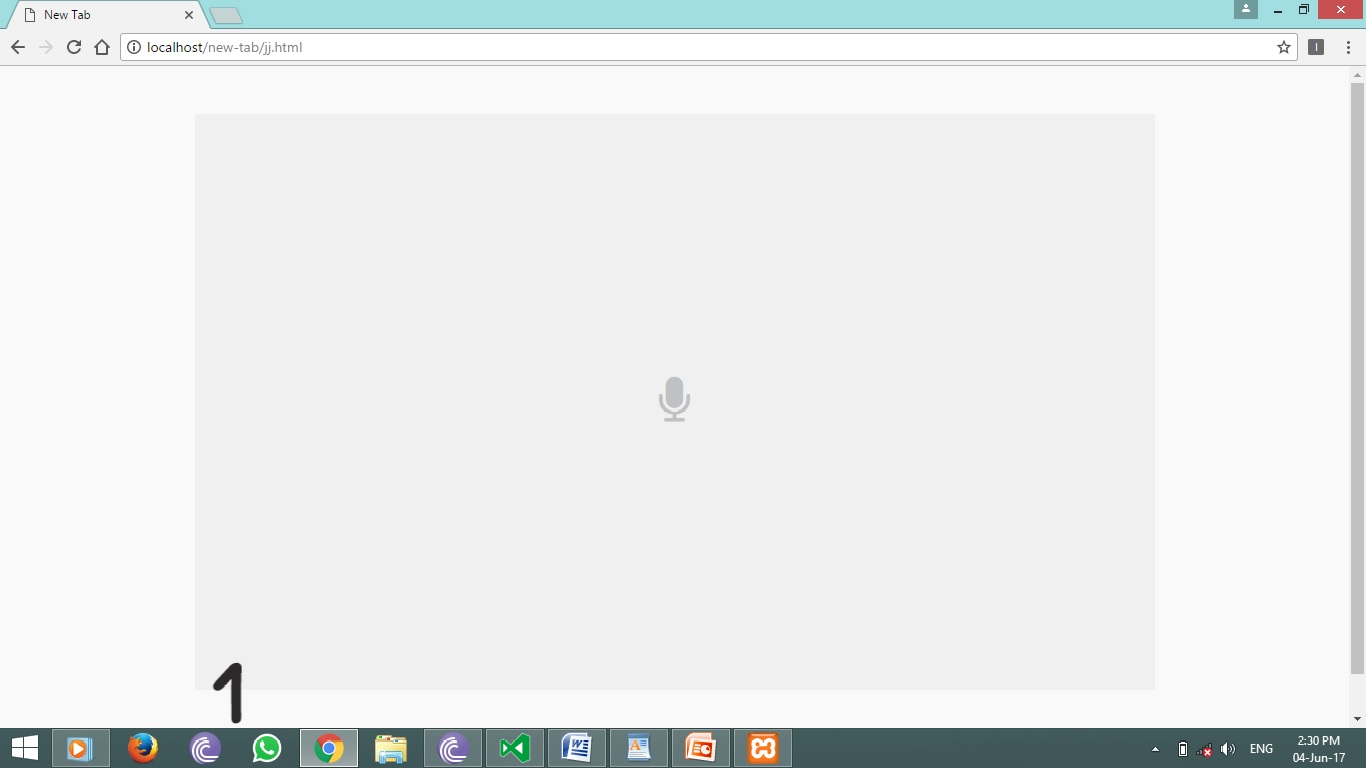
\includegraphics[width=\linewidth]{figures/screen1.jpg}
	\caption{Screen short 1}
	\label{fig:Screen short 1}
\end{figure}


\begin{figure}[ht]
	\centering
	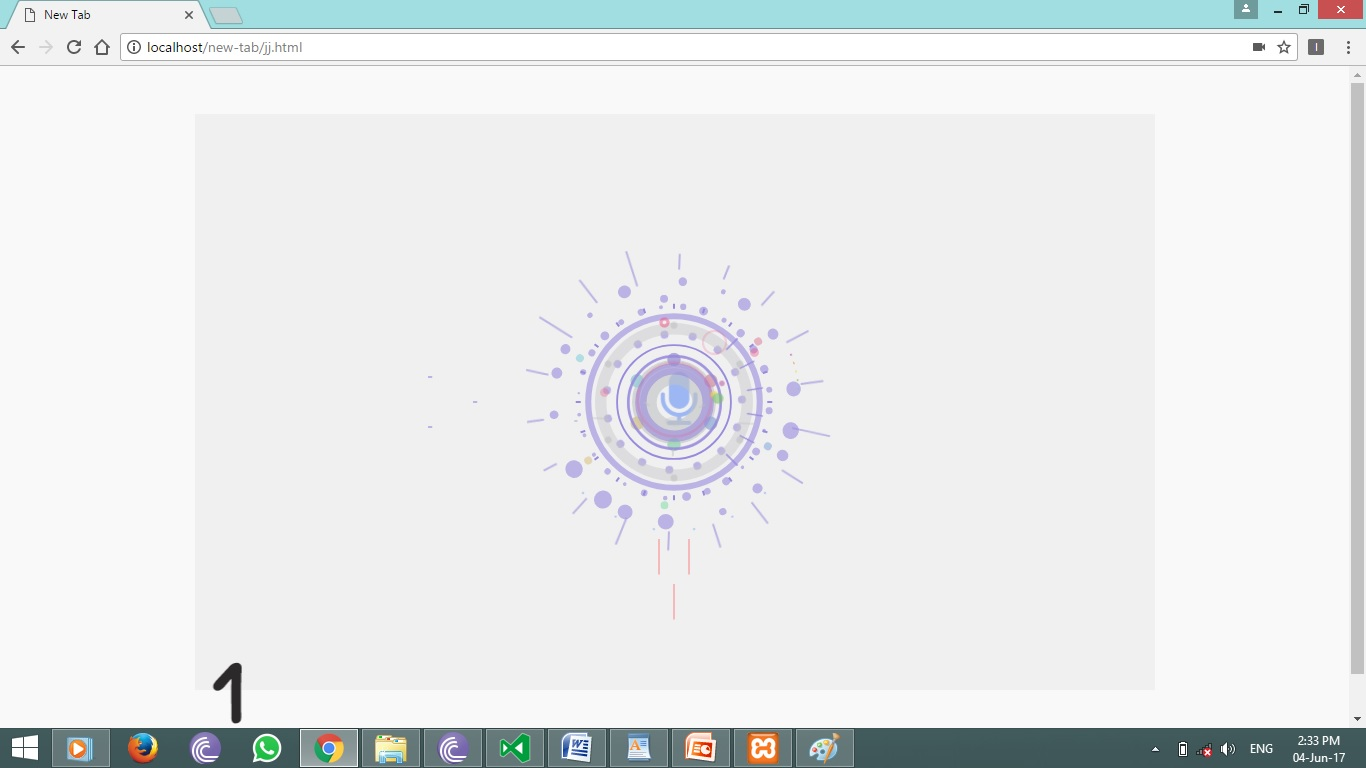
\includegraphics[width=\linewidth]{figures/screen2.jpg}
	\caption{Screen short 2}
	\label{fig:Screen short 2}
\end{figure}


\begin{figure}[ht]
	\centering
	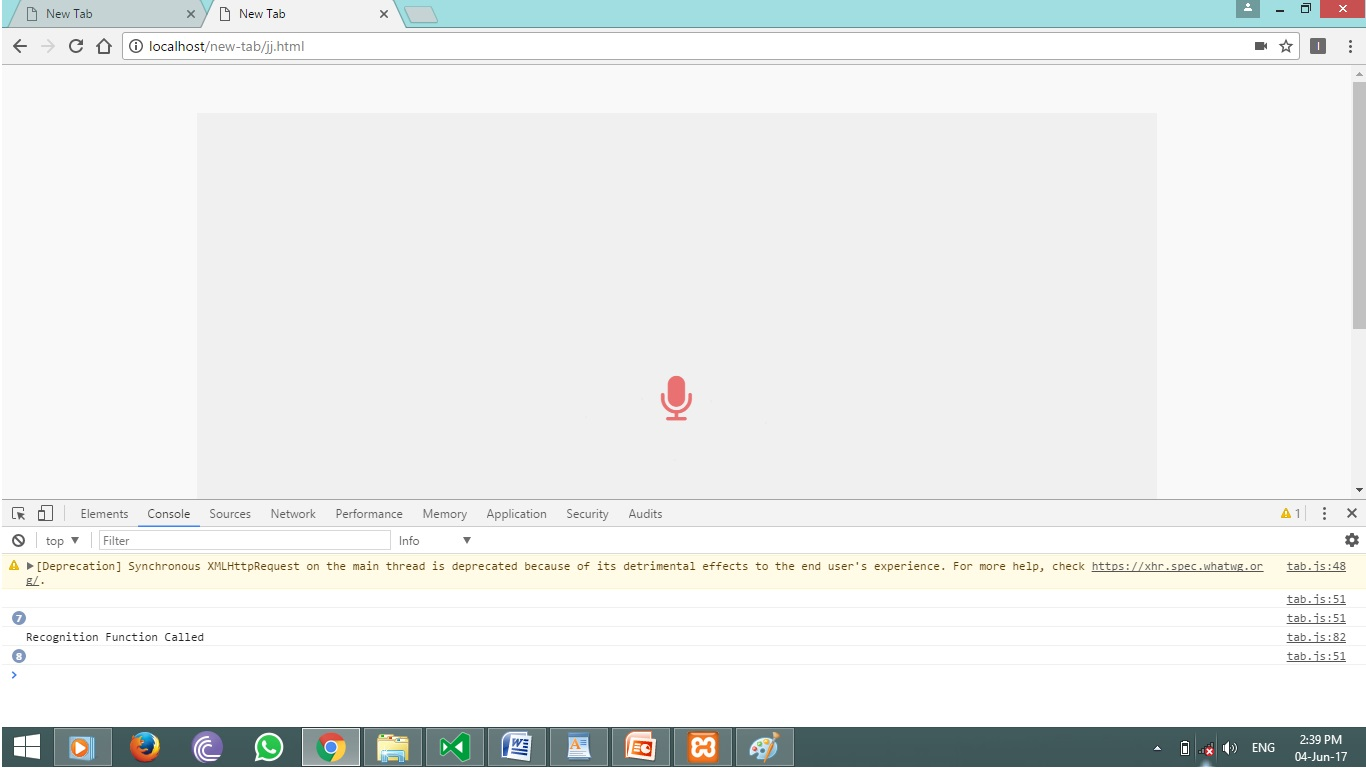
\includegraphics[width=\linewidth]{figures/screen3.jpg}
	\caption{Screen short 3}
	\label{fig:Screen short 3}
\end{figure}

\begin{figure}[ht]
	\centering
	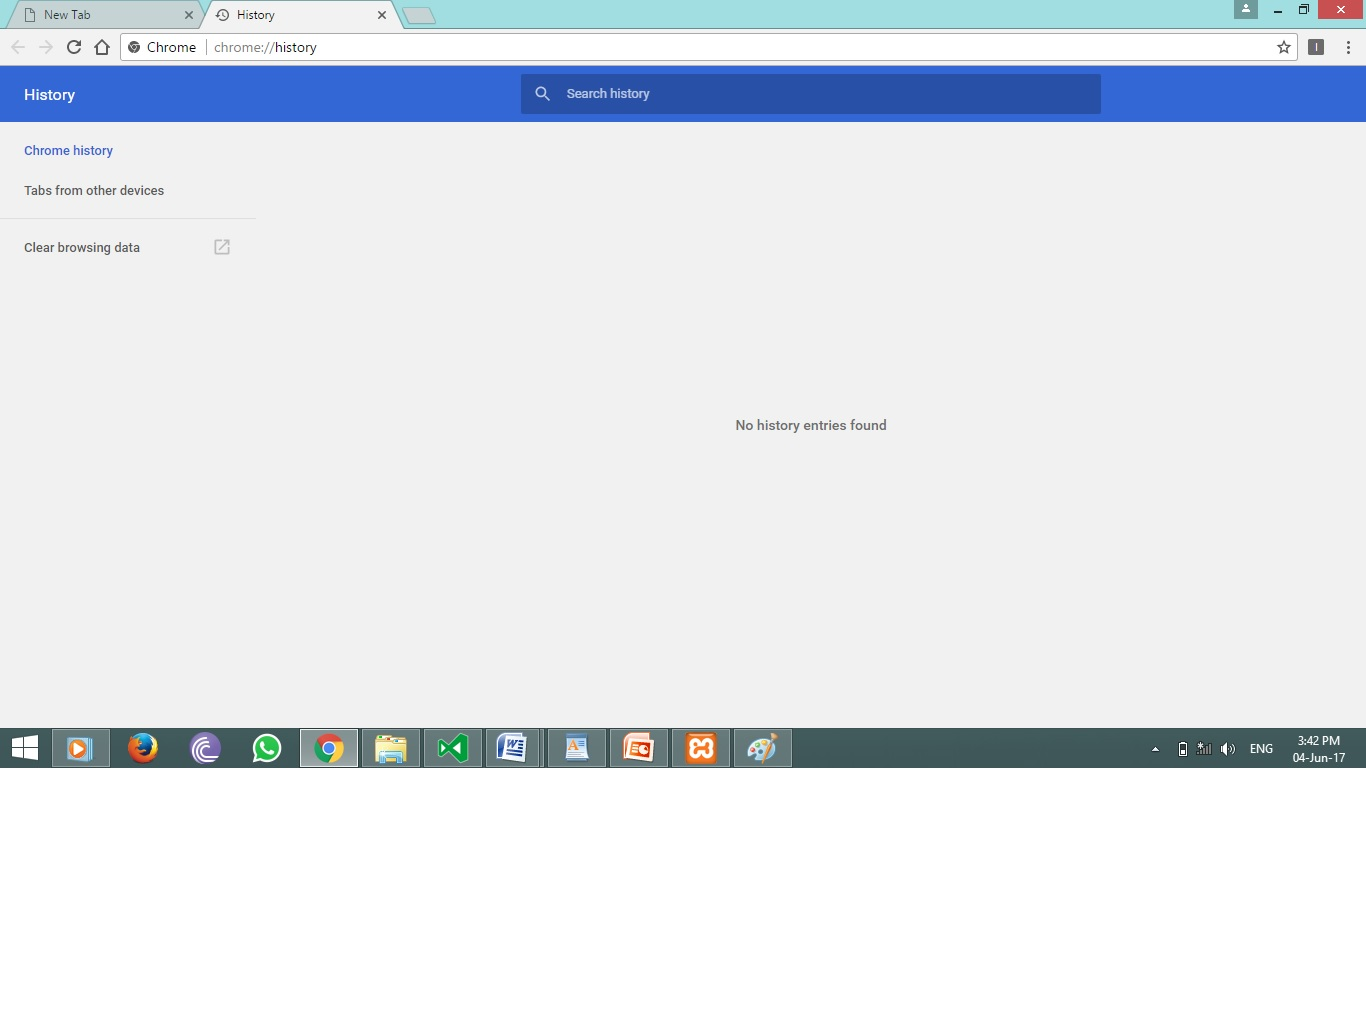
\includegraphics[width=\linewidth]{figures/screen4.jpg}
	\caption{Screen short 4}
	\label{fig:Screen short 4}
\end{figure}

\begin{figure}[ht]
	\centering
	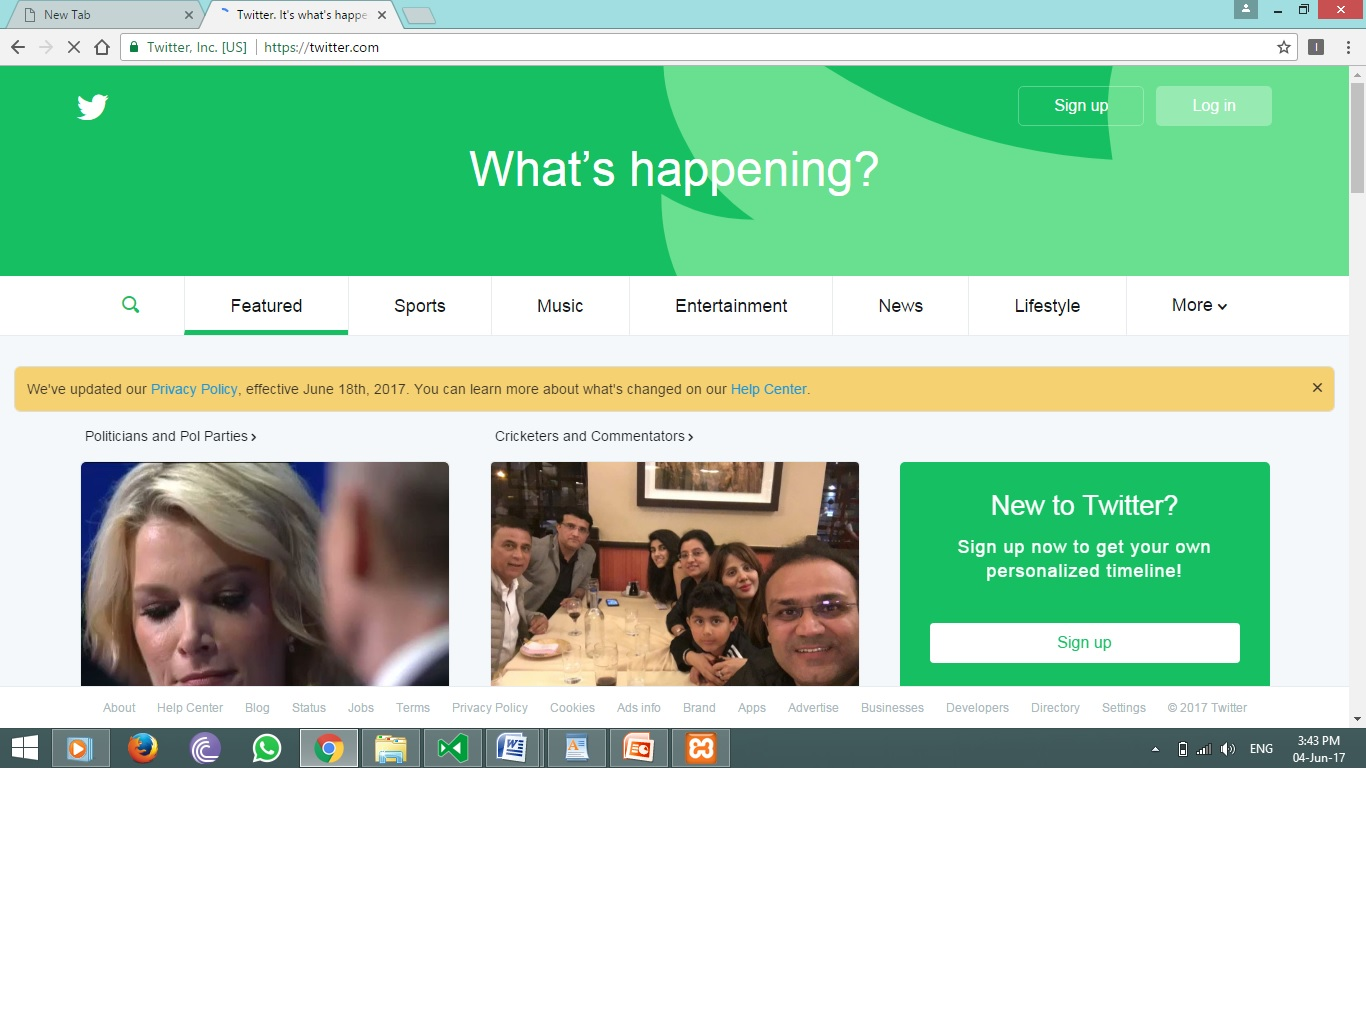
\includegraphics[width=\linewidth]{figures/screen5.jpg}
	\caption{Screen short 5}
	\label{fig:Screen short 5}
\end{figure}


\nocite{HTTPWikipedia}
\nocite{javahttpsessionStackoverflow}
\bibliographystyle{unsrt}
\bibliography{reference}

\end{document}